\documentclass[14pt]{extbook}
\usepackage{multicol, enumerate, enumitem, hyperref, color, soul, setspace, parskip, fancyhdr} %General Packages
\usepackage{amssymb, amsthm, amsmath, latexsym, units, mathtools} %Math Packages
\everymath{\displaystyle} %All math in Display Style
% Packages with additional options
\usepackage[headsep=0.5cm,headheight=12pt, left=1 in,right= 1 in,top= 1 in,bottom= 1 in]{geometry}
\usepackage[usenames,dvipsnames]{xcolor}
\usepackage{dashrule}  % Package to use the command below to create lines between items
\newcommand{\litem}[1]{\item#1\hspace*{-1cm}\rule{\textwidth}{0.4pt}}
\pagestyle{fancy}
\lhead{Progress Quiz 9}
\chead{}
\rhead{Version A}
\lfoot{9541-5764}
\cfoot{}
\rfoot{Summer C 2021}
\begin{document}

\begin{enumerate}
\litem{
Choose the equation of the function graphed below.
\begin{center}
    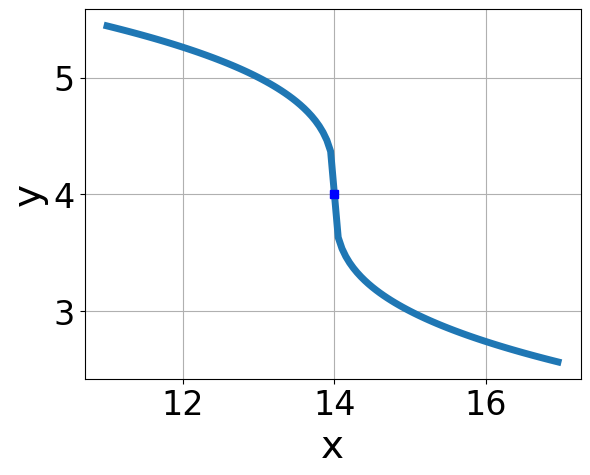
\includegraphics[width=0.5\textwidth]{../Figures/radicalGraphToEquationA.png}
\end{center}
\begin{enumerate}[label=\Alph*.]
\item \( f(x) = - \sqrt{x + 14} + 4 \)
\item \( f(x) = \sqrt{x + 14} + 4 \)
\item \( f(x) = - \sqrt{x - 14} + 4 \)
\item \( f(x) = \sqrt{x - 14} + 4 \)
\item \( \text{None of the above} \)

\end{enumerate} }
\litem{
Choose the equation of the function graphed below.
\begin{center}
    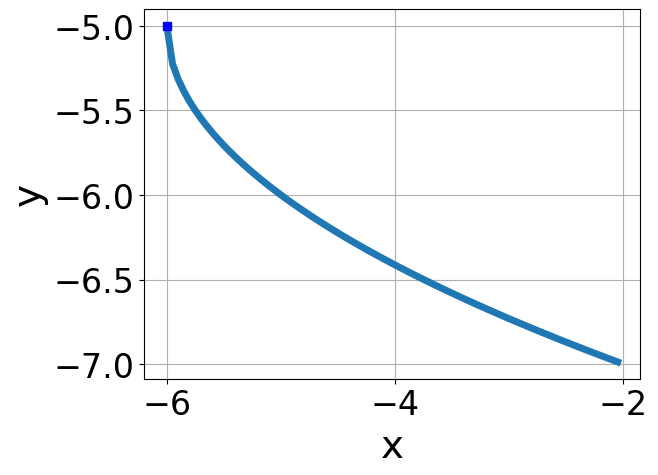
\includegraphics[width=0.5\textwidth]{../Figures/radicalGraphToEquationCopyA.png}
\end{center}
\begin{enumerate}[label=\Alph*.]
\item \( f(x) = - \sqrt{x + 6} - 5 \)
\item \( f(x) = - \sqrt{x - 6} - 5 \)
\item \( f(x) = \sqrt{x + 6} - 5 \)
\item \( f(x) = \sqrt{x - 6} - 5 \)
\item \( \text{None of the above} \)

\end{enumerate} }
\litem{
Solve the radical equation below. Then, choose the interval(s) that the solution(s) belongs to.\[ \sqrt{21 x^2 + 36} - \sqrt{-55 x} = 0 \]\begin{enumerate}[label=\Alph*.]
\item \( x_1 \in [1.26, 1.43] \text{ and } x_2 \in [-0.67,6.33] \)
\item \( \text{All solutions lead to invalid or complex values in the equation.} \)
\item \( x \in [-1.35,-1.29] \)
\item \( x \in [-1.29,-1.27] \)
\item \( x_1 \in [-1.35, -1.29] \text{ and } x_2 \in [-4.29,-0.29] \)

\end{enumerate} }
\litem{
Solve the radical equation below. Then, choose the interval(s) that the solution(s) belongs to.\[ \sqrt{-3 x + 2} - \sqrt{9 x - 8} = 0 \]\begin{enumerate}[label=\Alph*.]
\item \( x_1 \in [0.6, 0.71] \text{ and } x_2 \in [0.81,0.86] \)
\item \( x_1 \in [0.6, 0.71] \text{ and } x_2 \in [0.86,0.95] \)
\item \( x \in [0.7,0.94] \)
\item \( x \in [-0.52,-0.37] \)
\item \( \text{All solutions lead to invalid or complex values in the equation.} \)

\end{enumerate} }
\litem{
What is the domain of the function below?\[ f(x) = \sqrt[7]{-9 x - 8} \]\begin{enumerate}[label=\Alph*.]
\item \( \text{The domain is } (-\infty, a], \text{   where } a \in [-1.58, -0.89] \)
\item \( \text{The domain is } [a, \infty), \text{   where } a \in [-1.41, -0.9] \)
\item \( \text{The domain is } [a, \infty), \text{   where } a \in [-1.07, -0.53] \)
\item \( (-\infty, \infty) \)
\item \( \text{The domain is } (-\infty, a], \text{   where } a \in [-1.12, -0.1] \)

\end{enumerate} }
\litem{
Choose the graph of the equation below.\[ f(x) = \sqrt{x - 6} + 6 \]\begin{enumerate}[label=\Alph*.]
\begin{multicols}{2}\item 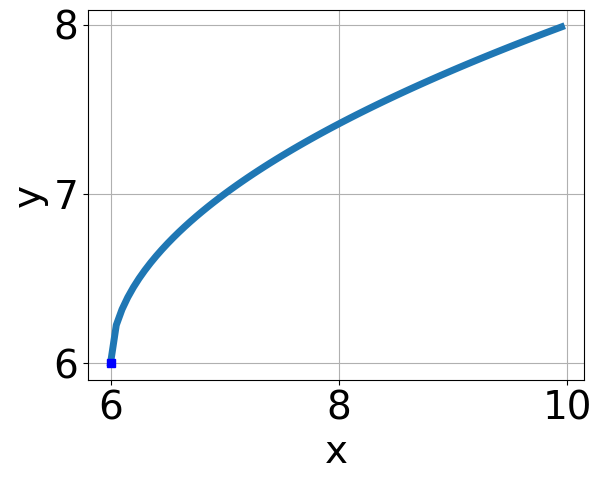
\includegraphics[width = 0.3\textwidth]{../Figures/radicalEquationToGraphAA.png}\item 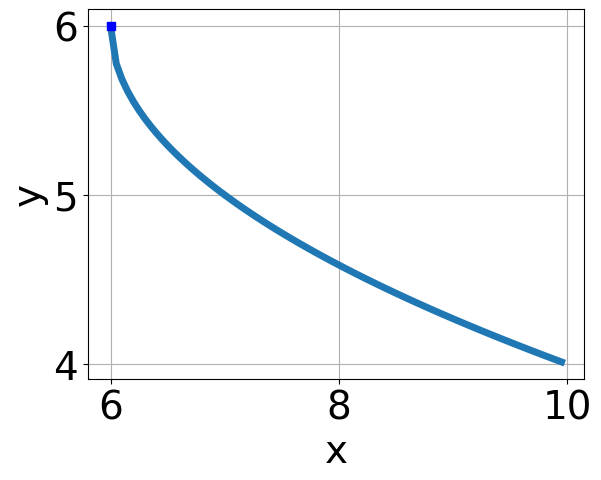
\includegraphics[width = 0.3\textwidth]{../Figures/radicalEquationToGraphBA.png}\item 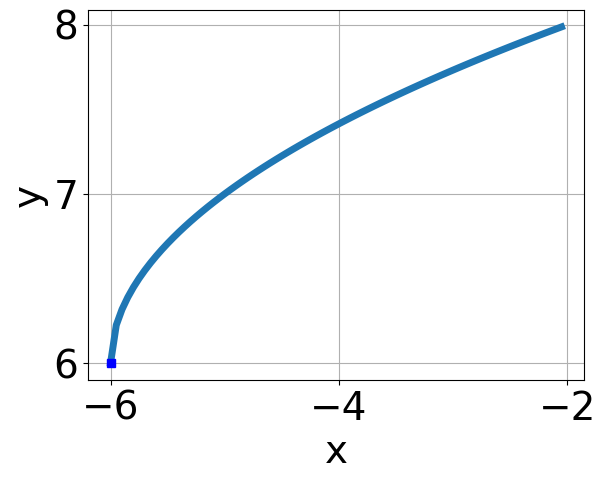
\includegraphics[width = 0.3\textwidth]{../Figures/radicalEquationToGraphCA.png}\item 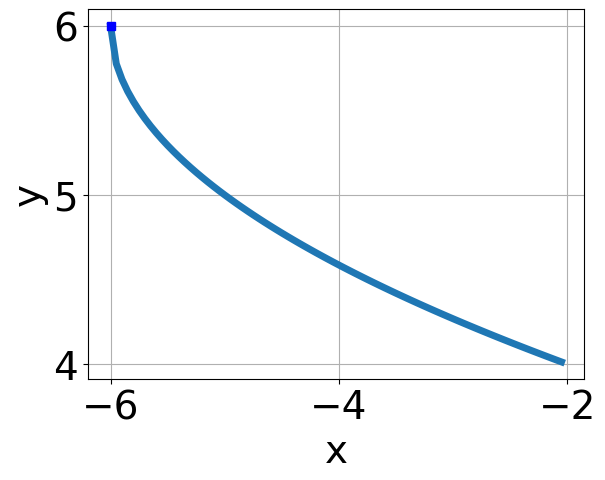
\includegraphics[width = 0.3\textwidth]{../Figures/radicalEquationToGraphDA.png}\end{multicols}\item None of the above.
\end{enumerate} }
\litem{
What is the domain of the function below?\[ f(x) = \sqrt[7]{8 x - 9} \]\begin{enumerate}[label=\Alph*.]
\item \( (-\infty, \infty) \)
\item \( \text{The domain is } (-\infty, a], \text{   where } a \in [1.03, 2.09] \)
\item \( \text{The domain is } (-\infty, a], \text{   where } a \in [0.88, 0.92] \)
\item \( \text{The domain is } [a, \infty), \text{   where } a \in [0.86, 1.12] \)
\item \( \text{The domain is } [a, \infty), \text{   where } a \in [1.11, 1.38] \)

\end{enumerate} }
\litem{
Solve the radical equation below. Then, choose the interval(s) that the solution(s) belongs to.\[ \sqrt{18 x^2 + 40} - \sqrt{-61 x} = 0 \]\begin{enumerate}[label=\Alph*.]
\item \( x_1 \in [-3.63, -1.99] \text{ and } x_2 \in [-3.89,0.11] \)
\item \( x \in [-1.96,-0.45] \)
\item \( x_1 \in [-0.22, 1.61] \text{ and } x_2 \in [2.5,3.5] \)
\item \( \text{All solutions lead to invalid or complex values in the equation.} \)
\item \( x \in [-3.63,-1.99] \)

\end{enumerate} }
\litem{
Choose the graph of the equation below.\[ f(x) = \sqrt[3]{x + 12} - 3 \]\begin{enumerate}[label=\Alph*.]
\begin{multicols}{2}\item 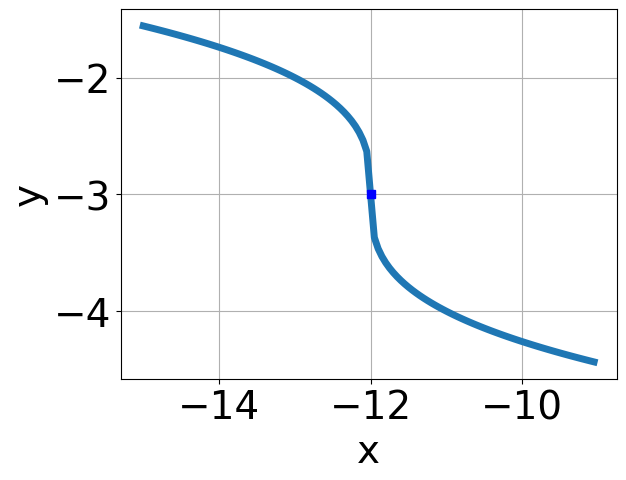
\includegraphics[width = 0.3\textwidth]{../Figures/radicalEquationToGraphCopyAA.png}\item 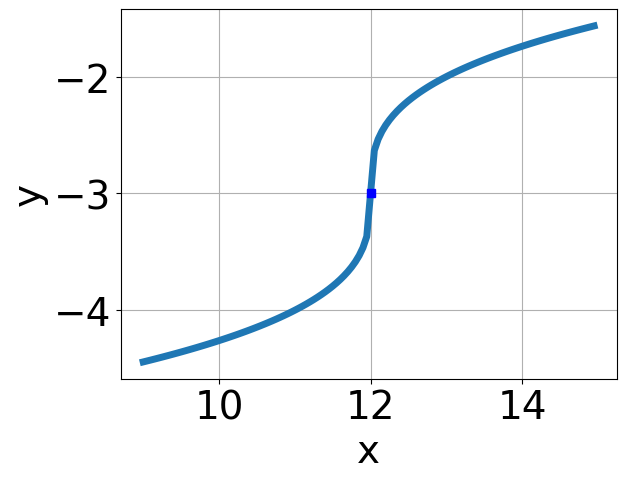
\includegraphics[width = 0.3\textwidth]{../Figures/radicalEquationToGraphCopyBA.png}\item 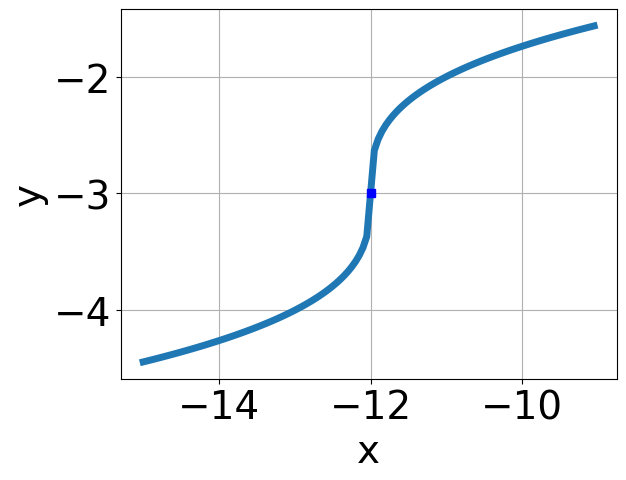
\includegraphics[width = 0.3\textwidth]{../Figures/radicalEquationToGraphCopyCA.png}\item 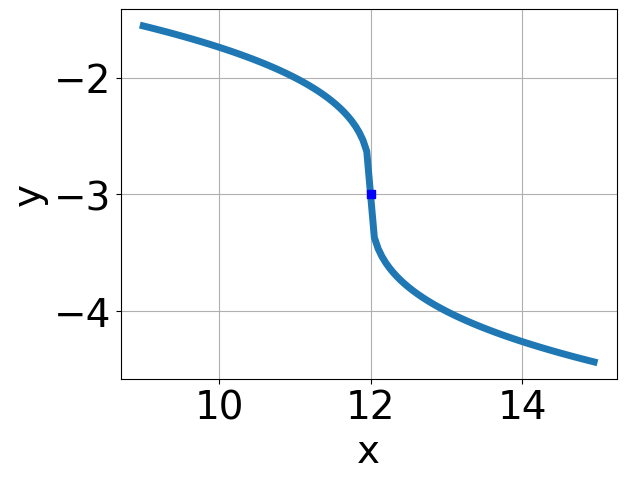
\includegraphics[width = 0.3\textwidth]{../Figures/radicalEquationToGraphCopyDA.png}\end{multicols}\item None of the above.
\end{enumerate} }
\litem{
Solve the radical equation below. Then, choose the interval(s) that the solution(s) belongs to.\[ \sqrt{7 x + 5} - \sqrt{-3 x - 9} = 0 \]\begin{enumerate}[label=\Alph*.]
\item \( x_1 \in [-3.4, -2.8] \text{ and } x_2 \in [-2.71,4.29] \)
\item \( x_1 \in [-1.6, -0.3] \text{ and } x_2 \in [-2.71,4.29] \)
\item \( x \in [-1.6,-0.3] \)
\item \( \text{All solutions lead to invalid or complex values in the equation.} \)
\item \( x \in [-1.1,0.5] \)

\end{enumerate} }
\end{enumerate}

\end{document}